\documentclass[8pt,a4paper]{article}

\usepackage{atbegshi}
\AtBeginShipoutFirst{\special{pdf:tounicode EUC-UCS2}}


%空白の設定
\usepackage{geometry}
\geometry{left=20truemm, right=20truemm, top=15truemm, bottom=20truemm}


%行間の設定
\renewcommand{\baselinestretch}{1.1}

\makeatletter
\newcommand{\figcaption}[1]{\def\@captype{figure}\caption{#1}}
\newcommand{\tblcaption}[1]{\def\@captype{table}\caption{#1}}
\makeatother
%コマンドの定義
\newcommand{\pcl}{\partial}
\newcommand{\bsm}{\boldsymbol}
\newcommand{\bm}{\boldsymbol}
\newcommand{\tr}{\mathrm{tr}}
\newcommand{\udl}{\underline}

\usepackage[nottoc]{tocbibind} 
\usepackage{booktabs}
\usepackage[dvipdfmx]{graphicx}
\usepackage{amsmath, amssymb}
\usepackage{txfonts}
\usepackage{wrapfig}
\usepackage{ascmac}
\usepackage{booktabs}
\usepackage{tabularx}
\usepackage{url}
\usepackage{color}
\usepackage{scalerel}
\usepackage{subfigure}

\DeclareMathOperator*{\assem}{\scalerel*{\textsf{A}}{\sum}}
%\usepackage[refeq, refpage, japanese]{nomencl}
%\makenomenclature

\setcounter{tocdepth}{4}
\setcounter{secnumdepth}{3}
\newcommand{\todayd}{\the\year/\the\month/\the\day}


\begin{document} 

\begin{center}
	{\Large 安定化有限要素法による移流拡散方程式 (convection-diffusion equation) ソルバーの検証} \\
\end{center}

%\begin{flushright}
%\begin{center}
%	{\Large Naoto Mitsume}
%\end{center}
%\end{flushright}    

\section{支配方程式と離散化後方程式}
\subsection*{定常解析 (steady analysis)}
支配方程式:
\begin{align}
	a \bsm{v} \cdot \nabla u + \nabla \cdot \left( -k \nabla u \right) = f
\end{align}

\noindent
重み付き残差式:
\begin{align}
	\begin{split}
		&\int_{\Omega} N_i a_h \bsm{v}_h \cdot \nabla u_h d\Omega + \int_{\Omega} \nabla N_i \cdot \left( k_h \nabla u_h \right) d\Omega - \int_{\Omega} N_i f_h d\Omega \\
		&\quad + \sum_e \int_{\Omega_e} \tau_e \left( a_h \bsm{v}_h \cdot \nabla N_i \right) \left( a_h \bsm{v}_h \cdot \nabla u_h + \nabla \cdot \left( -k \nabla u_h \right) - f \right) d\Omega = 
		\int_{\pcl \Omega^q} N_i k_h \nabla u_h \cdot \bsm{n} d\Gamma 
	\end{split}
\end{align}
\begin{align}
	\tau_e &= \frac{h_e}{2|\bsm{v}|} \left( \frac{1}{\tanh \alpha} - \frac{1}{\alpha} \right), \qquad
	\alpha = \frac{|\bsm{v}| h_e}{2k}, \qquad
	h_e = \left( \int_{\Omega_e} d\Omega \right)^{\frac{1}{3}}
\end{align}

\noindent
線形方程式:
\begin{align}
	\udl{\bsm{K}} \ \udl{\bsm{u}} = \udl{\bsm{f}}
\end{align}
\begin{align}
	\udl{K}_{ij} &= \sum_e \int_{\Omega_e} \left[ a_h N_i \left( \bsm{v}_h \cdot \nabla N_j \right) + k_h \nabla N_i \cdot \nabla N_j + \tau_e (a_h)^2 \left( \bsm{v}_h \cdot \nabla N_i \right) \left( \bsm{v}_h \cdot \nabla N_j \right) \right] d\Omega \\
	\udl{f}_i    &= \sum_e \int_{\Omega_e} \left[ f_h N_i + f_h a_h \bsm{v}_h \cdot \nabla N_i \right] d\Omega + \sum_s \int_{\pcl \Omega^q_s} \left( k_h \nabla u_h  \cdot \bsm{n} \right) N_i d\Gamma 
\end{align}
\begin{itemize}
	\item 下付き添字$\cdot_h$は有限要素によって分布を離散化された物理量 ($a_h = \sum_i N_i a_i$, $a_i$は節点$i$での$a$の値)
	\item 安定化項中の拡散に関する項は二階微分を含み、1次要素では$0$となるため消去
\end{itemize}

\subsection*{非定常解析 (non-steady analysis)}
\begin{align}
	a \left( \frac{\pcl u}{\pcl t} + \bsm{v} \cdot \nabla u \right) + \nabla \cdot \left( -k \nabla u \right) = f
\end{align}

\begin{align}
	\begin{split}
		&\int_{\Omega} N_i a_h \frac{\pcl u_h}{\pcl t} d\Omega + \int_{\Omega} N_i a_h \bsm{v}_h \cdot \nabla u_h d\Omega + \int_{\Omega} \nabla N_i \cdot \left( k_h \nabla u_h \right) d\Omega - \int_{\Omega} N_i f_h d\Omega \\
		&\quad + \sum_e \int_{\Omega_e} \tau_e \left( a_h \bsm{v}_h \cdot \nabla N_i \right) \left( a_h \frac{\pcl u_h}{\pcl t} + a_h \bsm{v}_h \cdot \nabla u_h + \nabla \cdot \left( -k \nabla u_h \right) - f \right) d\Omega = 
		\int_{\pcl \Omega^q} N_i k_h \nabla u_h \cdot \bsm{n} d\Gamma 
	\end{split}
\end{align}
\begin{align}
	\tau_e &= \left\{ \left( \frac{2}{\Delta t} \right)^2 + \left( \frac{2 |\bsm{v}|}{h_e} \right)^2 + \left( \frac{4k}{a h^2}^2 \right) \right\}^{-\frac{1}{2}}
\end{align}

\noindent
線形方程式 (時間方向離散化が陰的 Euler 法の場合):
\begin{align}
	\udl{\bsm{K}} \ \udl{\bsm{u}}^{n+1} = \udl{\bsm{f}}
\end{align}
\begin{align}
	\udl{K}_{ij} &= \sum_e \int_{\Omega_e} \left[ \frac{1}{\Delta t} a_h N_i N_j + a_h N_i \left( \bsm{v}_h \cdot \nabla N_j \right) + k_h \nabla N_i \cdot \nabla N_j +  \frac{1}{\Delta t} \tau_e (a_h)^2 \left( \bsm{v}_h \cdot \nabla N_i \right) N_j + \tau_e (a_h)^2 \left( \bsm{v}_h \cdot \nabla N_i \right) \left( \bsm{v}_h \cdot \nabla N_j \right) \right] d\Omega \\
	\udl{f}_i    &= \sum_e \int_{\Omega_e} \left[ \frac{1}{\Delta t} u^n_h N_i + f_h N_i + \frac{1}{\Delta t} \tau_e u^n_h (a_h)^2 \bsm{v}_h \cdot \nabla N_i + f_h a_h \bsm{v}_h \cdot \nabla N_i \right] d\Omega + \sum_s \int_{\pcl \Omega^q_s} \left( k_h \nabla u_h  \cdot \bsm{n} \right) N_i d\Gamma 
\end{align}
\begin{itemize}
	\item 安定化パラメータ $\tau_e$ は文献\cite{hughes1989new}のものを使用 ($a$や$k$が空間的に一様でない場合も適用できるかは未知)
\end{itemize}
\clearpage

\section{創成解による精度検証}
開発したソルバーを創成解を用いて精度検証する。解析対象領域は $0 \leq x \leq 10, 0 \leq y \leq 10, 0 \leq z \leq 10$ の正立方体状の領域で、創成解の値を用いて全面に Dirichlet 境界条件を課す。また、$h$は要素の代表長さとする。

本精度検証では、基本的に以下の8パターンの解析を行う。六面体一次要素は正立方格子状に配置する。四面体要素は六面体要素を6分割し生成する。
\begin{itemize}
	\item 六面体一次要素 ($1/h=1$, 総節点数: 1{,}331, 総要素数: 1{,}000)
	\item 六面体一次要素 ($1/h=2$, 総節点数: 9{,}261, 総要素数: 8{,}000)
	\item 六面体一次要素 ($1/h=4$, 総節点数: 68{,}921, 総要素数: 64{,}000)
	\item 六面体一次要素 ($1/h=8$, 総節点数: 531{,}441, 総要素数: 512{,}000)
	\item 四面体一次要素 ($1/h=1$, 総節点数: 1{,}331, 総要素数: 6{,}000)
	\item 四面体一次要素 ($1/h=2$, 総節点数: 9{,}261, 総要素数: 48{,}000)
	\item 四面体一次要素 ($1/h=4$, 総節点数: 68{,}921, 総要素数: 384{,}000)
	\item 四面体一次要素 ($1/h=8$, 総節点数: 531{,}441, 総要素数: 3{,}072{,}000)
\end{itemize}
また、数値積分点は $3\times 3 \times 3 = 27$点用いる。四面体要素は六面体要素上に定義される積分点を写像し積分を行う。

\subsection{定常解析}
本項では以下の創成解を用いる。
\begin{align}
	u (\bsm{x}) &= \sin \left( 0.25 x \right) \sin \left( 0.5 y \right) \sin z 
\end{align}

\subsubsection{係数一定の拡散方程式}
\begin{align}
	a &= 0 \\
	\bsm{v} (\bsm{x}) &= 0 \\
	k (\bsm{x}) &= 1
\end{align}
\begin{align}
	f (\bsm{x}) &= -1.1875 \sin \left( 0.25 x \right) \sin \left( 0.5 y \right) \sin z 
\end{align}
\begin{figure}[h!!]
	\centering
	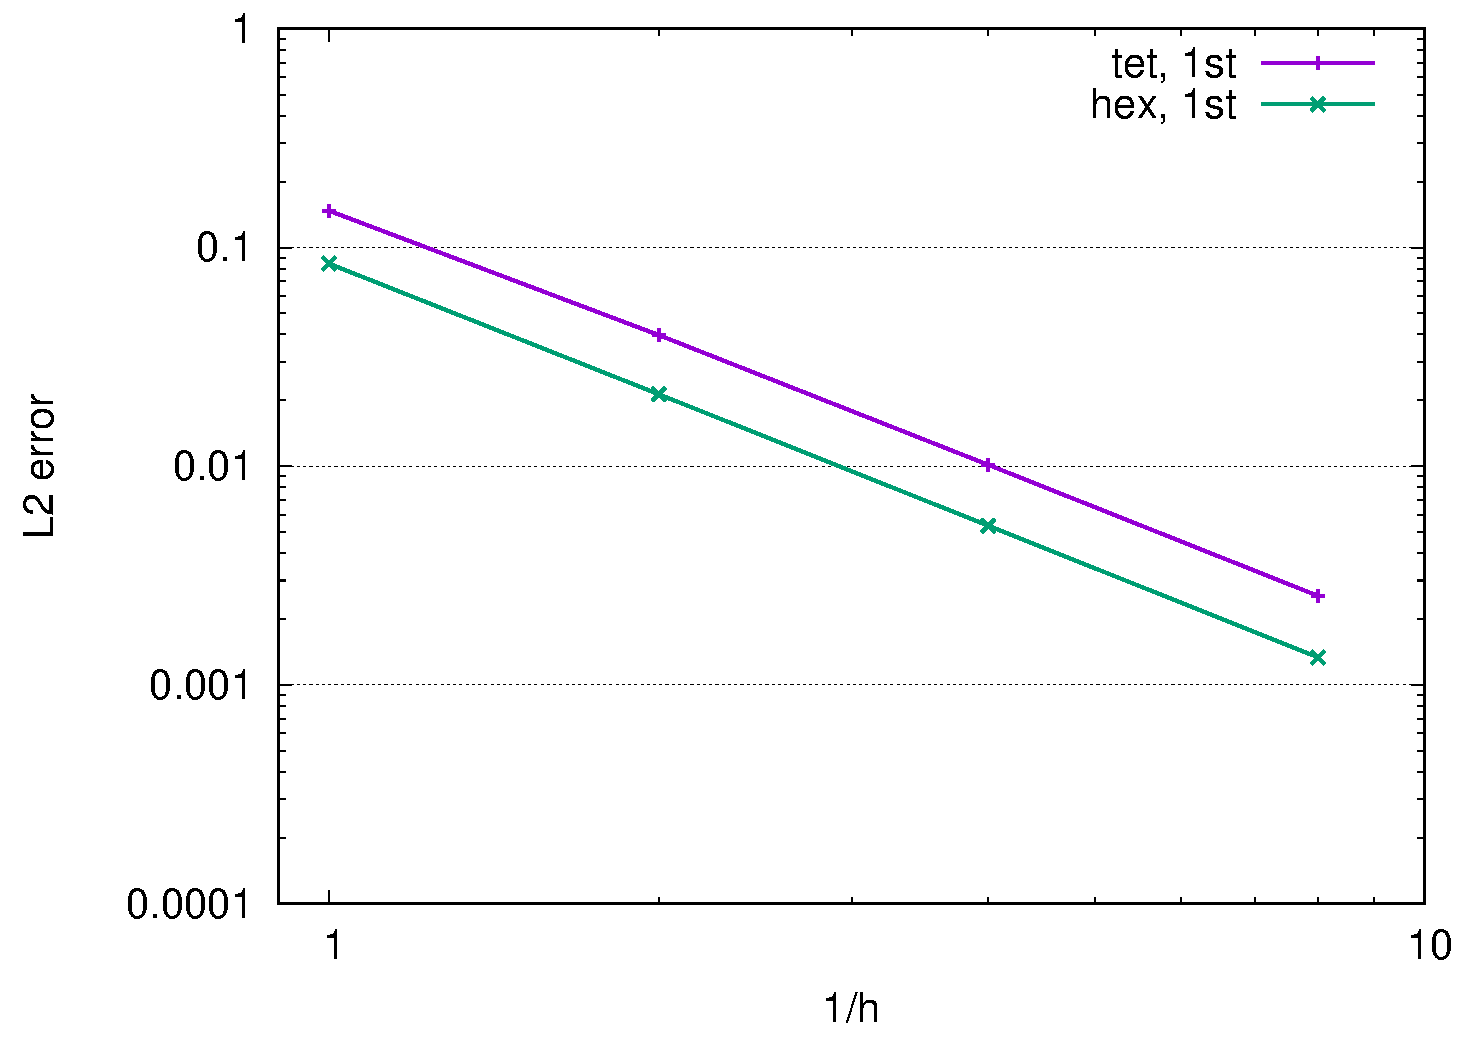
\includegraphics[width=10.0truecm]{pics/conv_diff_const.pdf}
	\caption{L2誤差: 定常・拡散方程式・係数一定}
	\label{fig:conv_diff_const}
\end{figure}

\subsubsection{係数非一定の拡散方程式}
\begin{align}
	a &= 0 \\
	\bsm{v} (\bsm{x}) &= 0 \\
	k (\bsm{x}) &= 2 + \sin x \sin \left( 0.5 y \right) \sin \left( 0.25 z \right)
\end{align}
\begin{align}
	\begin{split}
	f (\bsm{x}) &=  -1.1875 \sin \left( 0.25 x \right) \sin \left( 0.5 y \right) \sin z \\
		& \quad - \left\{     \cos x \sin \left( 0.5 y \right) \sin \left( 0.25 z \right) \right\} \left\{ 0.25 \cos \left( 0.25 x \right) \sin \left( 0.5 y \right) \sin z \right\} \\
		& \quad - \left\{0.5  \sin x \cos \left( 0.5 y \right) \sin \left( 0.25 z \right) \right\} \left\{ 0.5  \sin \left( 0.25 x \right) \cos \left( 0.5 y \right) \sin z \right\} \\
		& \quad - \left\{0.25 \sin x \sin \left( 0.5 y \right) \cos \left( 0.25 z \right) \right\} \left\{      \sin \left( 0.25 x \right) \sin \left( 0.5 y \right) \cos z \right\} 
	\end{split}
\end{align}
\begin{figure}[h!!]
	\centering
	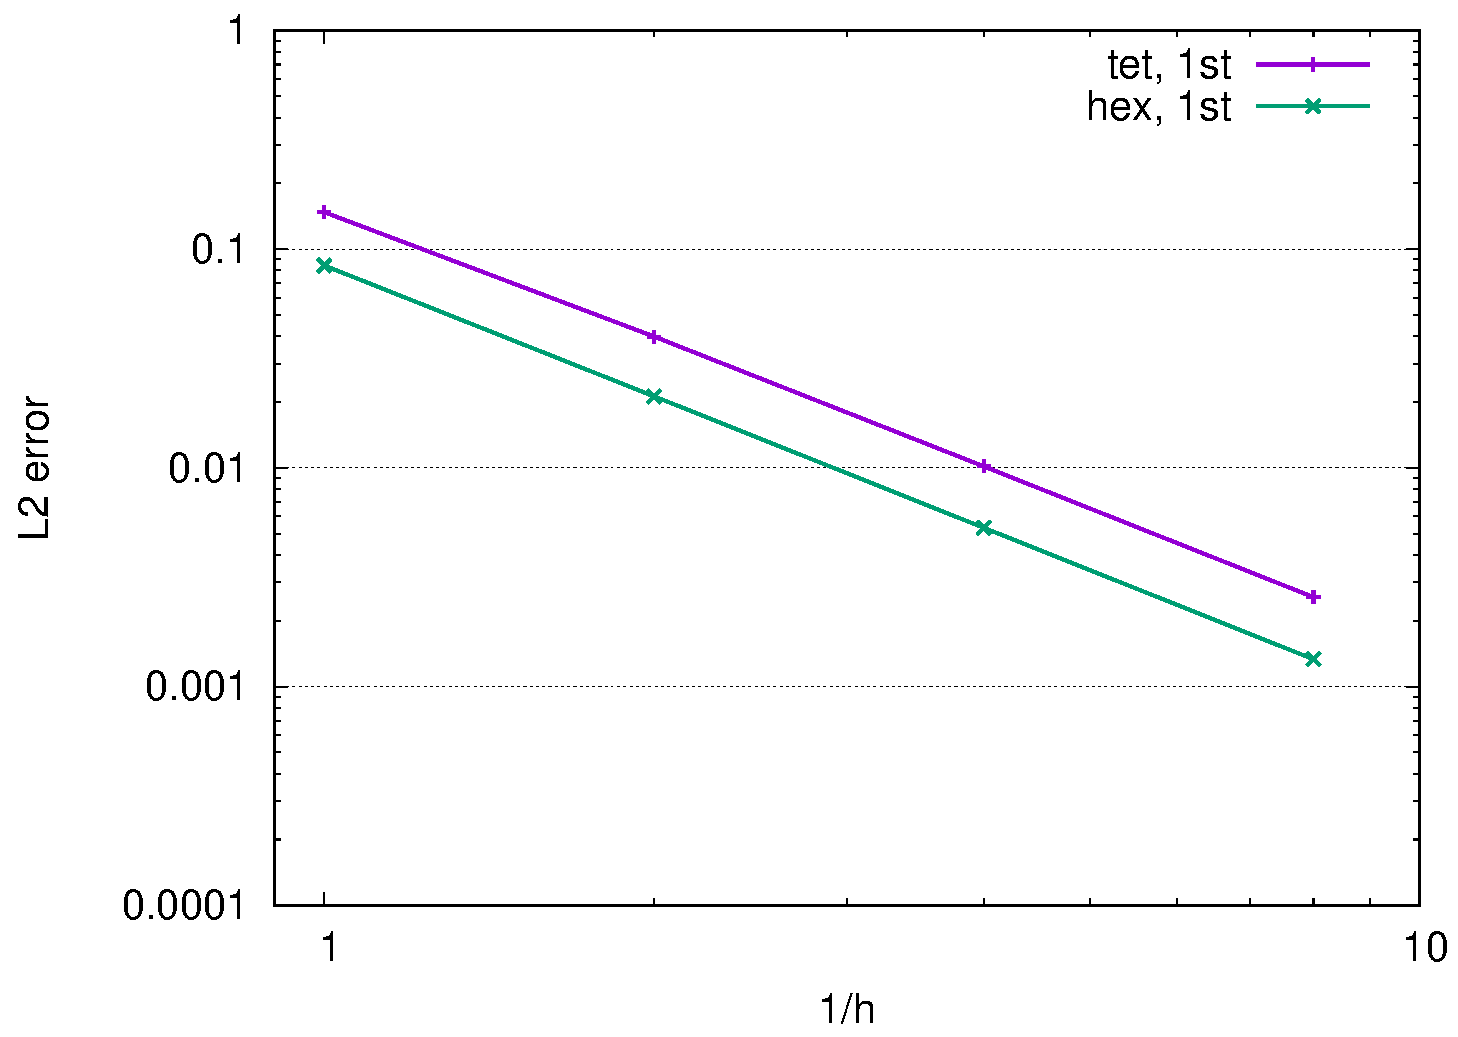
\includegraphics[width=10.0truecm]{pics/conv_diff_nonconst.pdf}
	\caption{L2誤差: 定常・拡散方程式・係数非一定}
	\label{fig:conv_diff_nonconst}
\end{figure}

\subsubsection{係数一定の移流拡散方程式}
\begin{align}
	a &= 1 \\
	\bsm{v} (\bsm{x}) &= \mathrm{Pe} \frac{1}{\sqrt{3}}\bsm{1} \\
	k (\bsm{x}) &= 1.0
\end{align}
\begin{align}
	\begin{split}
	f (\bsm{x}) &=  \mathrm{Pe} \frac{1}{\sqrt{3}} \left\{ 0.25 \cos \left( 0.25 x \right) \sin \left( 0.5 y \right) \sin z \right\} \\
		& \quad +\mathrm{Pe} \frac{1}{\sqrt{3}} \left\{ 0.5  \sin \left( 0.25 x \right) \cos \left( 0.5 y \right) \sin z \right\} \\
		& \quad +\mathrm{Pe} \frac{1}{\sqrt{3}} \left\{      \sin \left( 0.25 x \right) \sin \left( 0.5 y \right) \cos z \right\} \\
		& \quad - 1.1875 \sin \left( 0.25 x \right) \sin \left( 0.5 y \right) \sin z
	\end{split}
\end{align}
$\mathrm{Pe}$は Peclet 数を表す。なお、風上化を施さない場合は $\mathrm{Pe}$が$100$以上のケースで行列の反復求解が収束せず、計算が不可能であることを確認したが、本項では詳細な結果を省略する。

\clearpage

\begin{figure}[h!!]
	\centering
	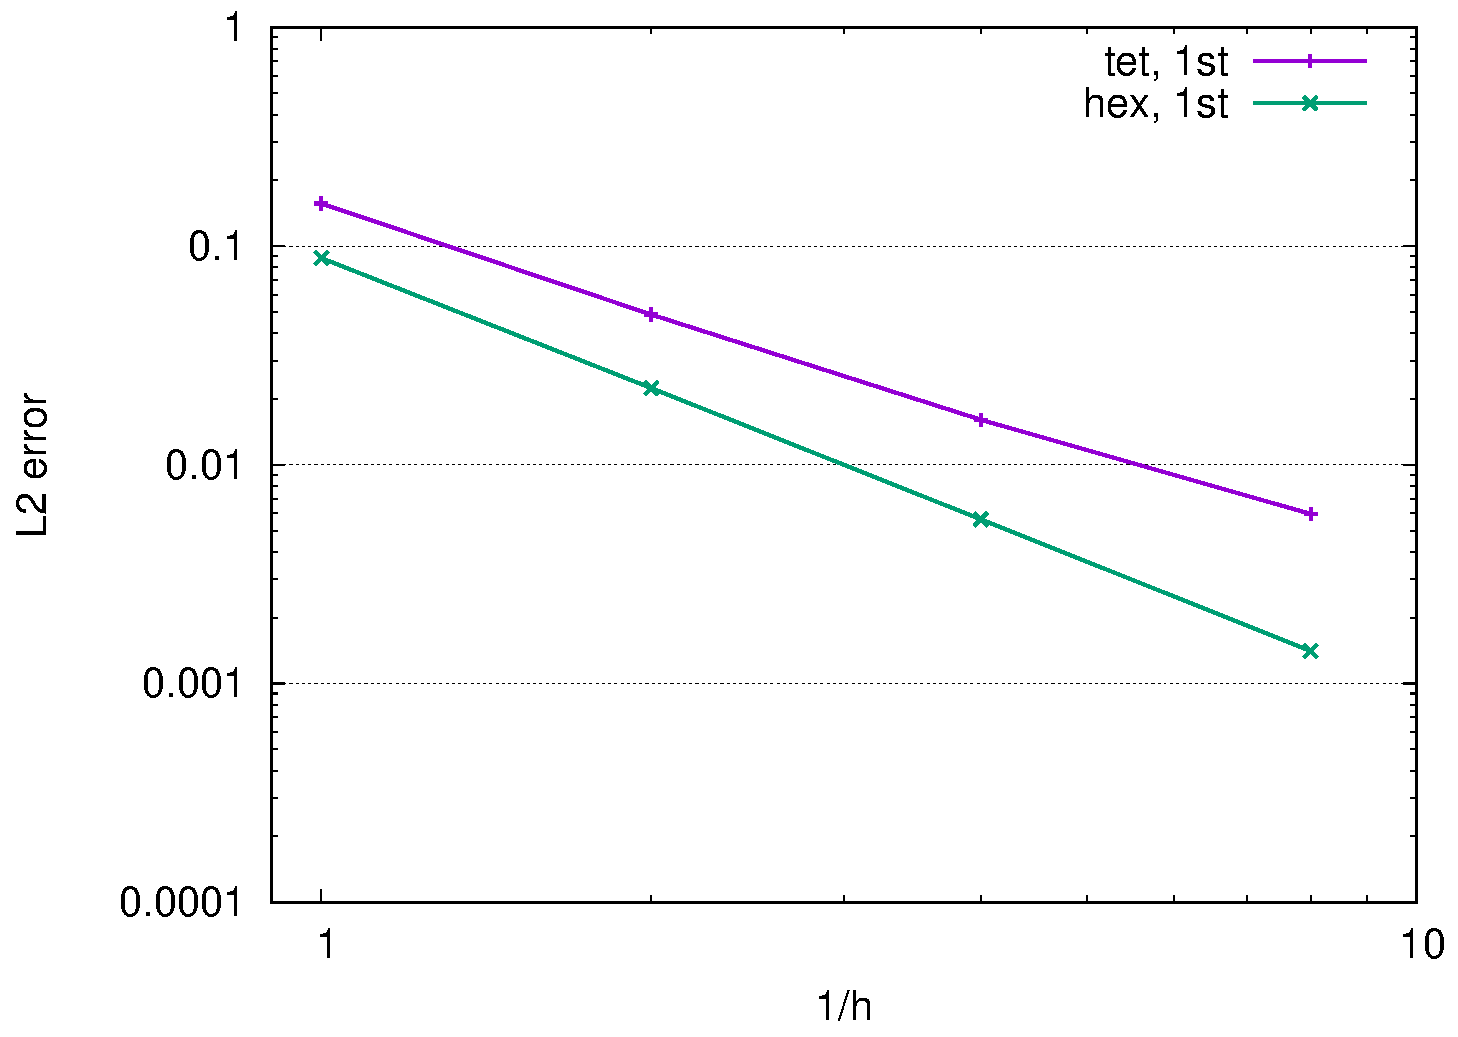
\includegraphics[width=10.0truecm]{pics/conv_convdiff_const_pe1.pdf}
	\caption{L2誤差: 定常・移流拡散方程式・係数一定・$\mathrm{Pe} = 1$}
	\label{fig:conv_convdiff_const_pe1}
\end{figure}
\begin{figure}[h!!]
	\centering
	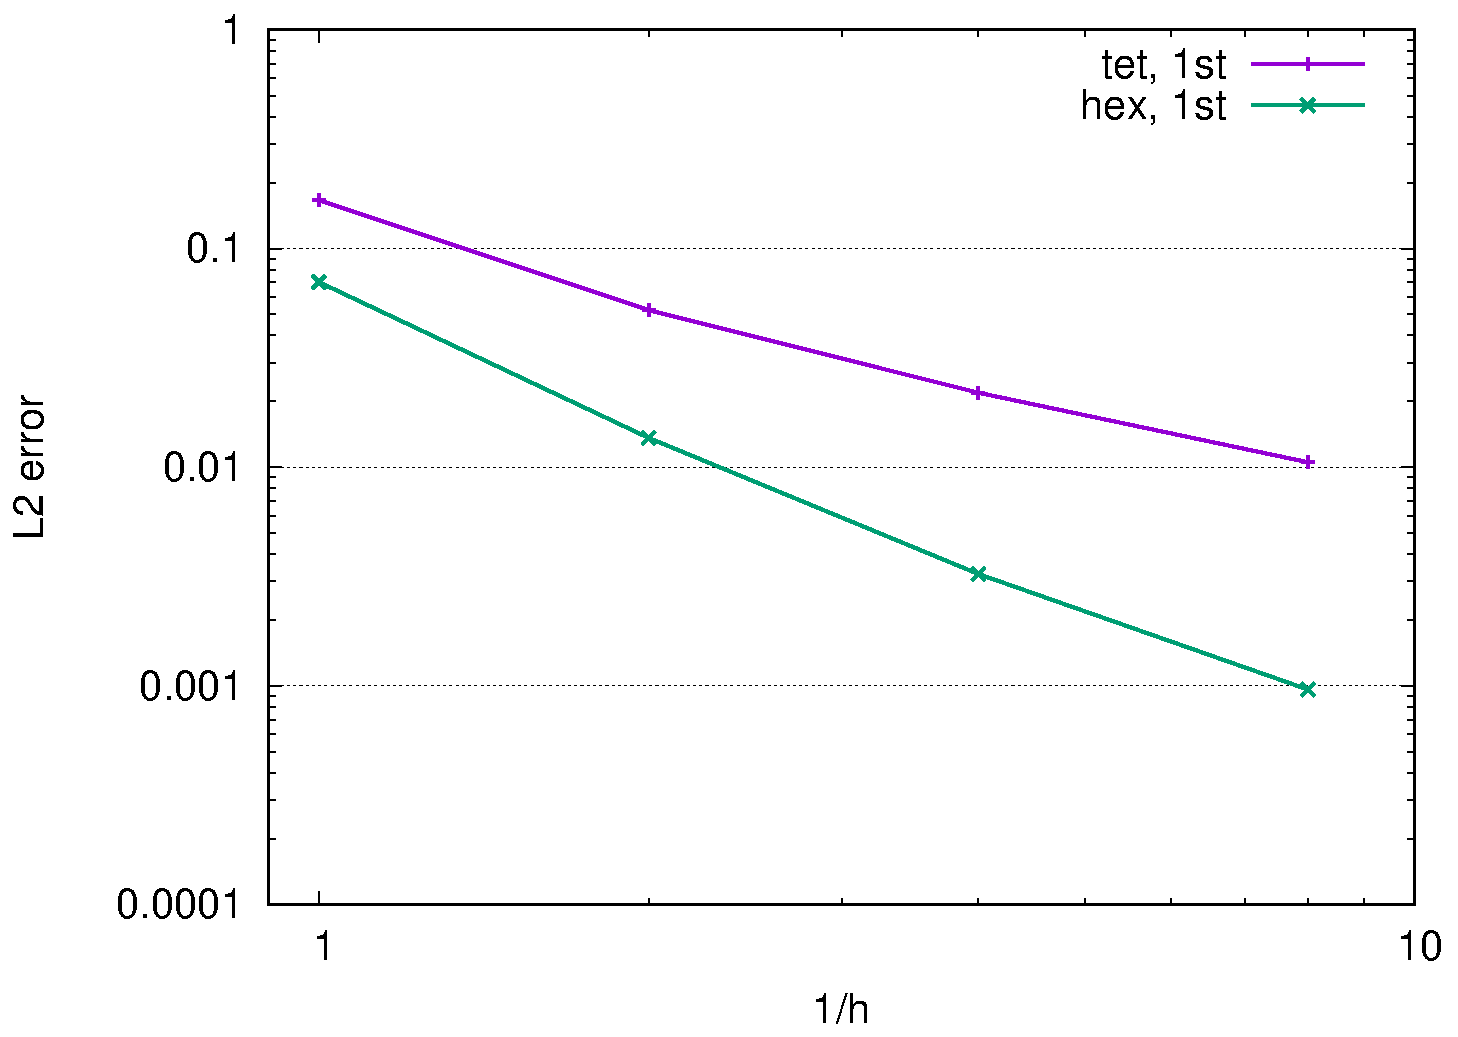
\includegraphics[width=10.0truecm]{pics/conv_convdiff_const_pe100.pdf}
	\caption{L2誤差: 定常・移流拡散方程式・係数一定・$\mathrm{Pe} = 100$}
	\label{fig:conv_convdiff_const_pe100}
\end{figure}
\begin{figure}[h!!]
	\centering
	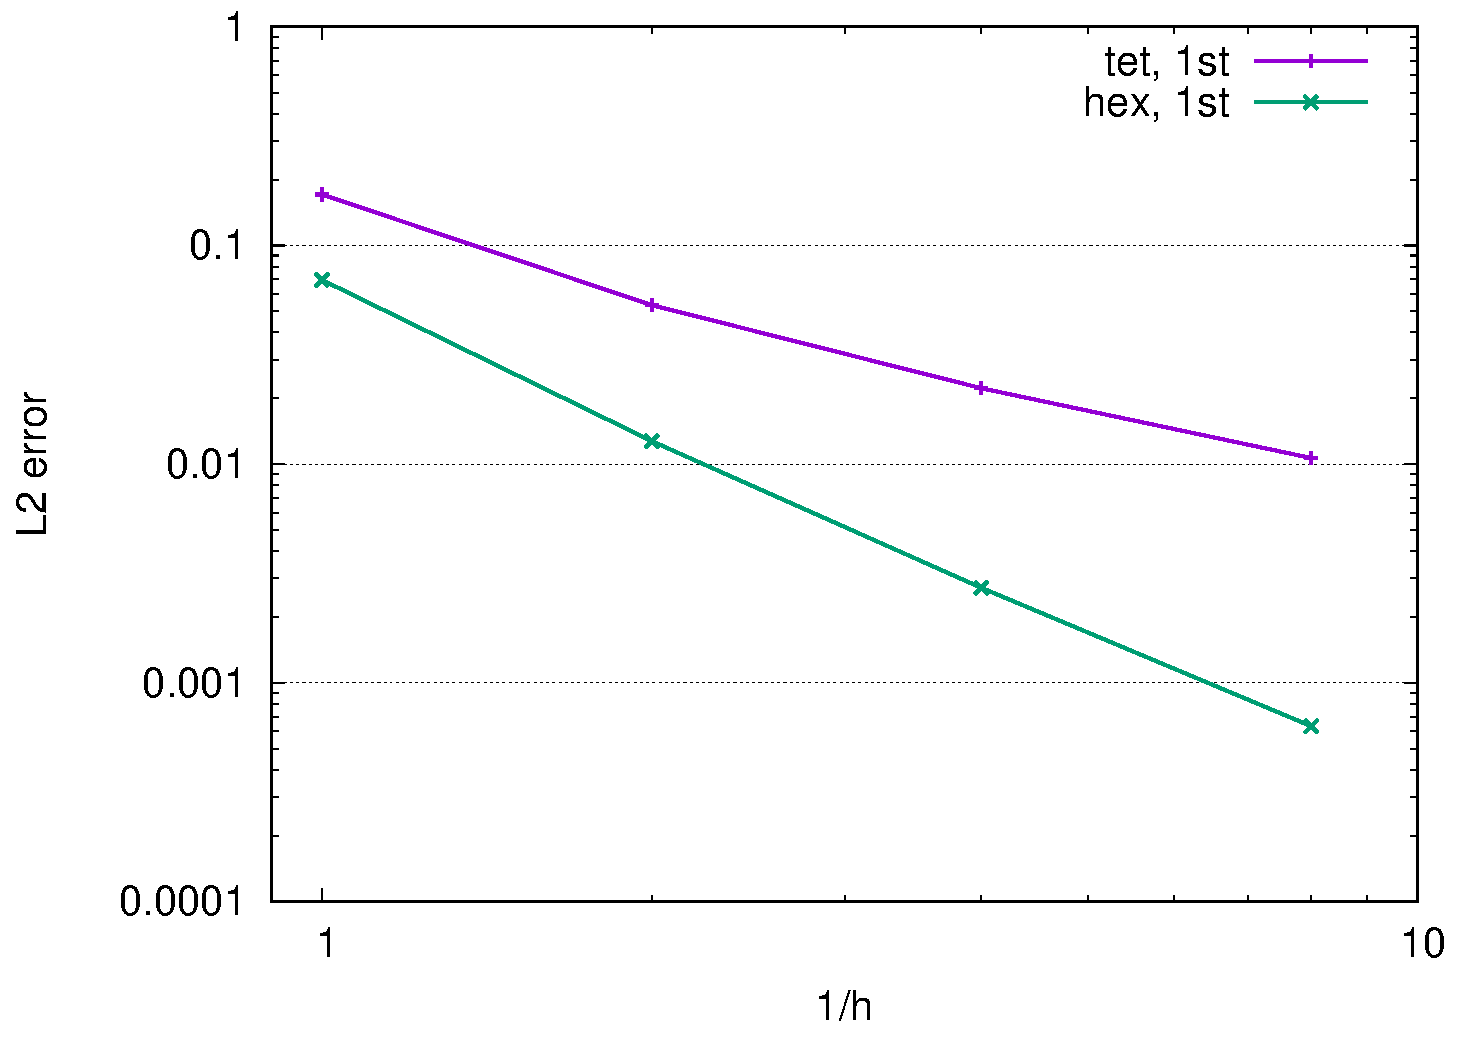
\includegraphics[width=10.0truecm]{pics/conv_convdiff_const_pe10000.pdf}
	\caption{L2誤差: 定常・移流拡散方程式・係数一定・$\mathrm{Pe} = 10{,}000$}
	\label{fig:conv_convdiff_const_pe10000}
\end{figure}
\begin{figure}[h!!]
	\centering
	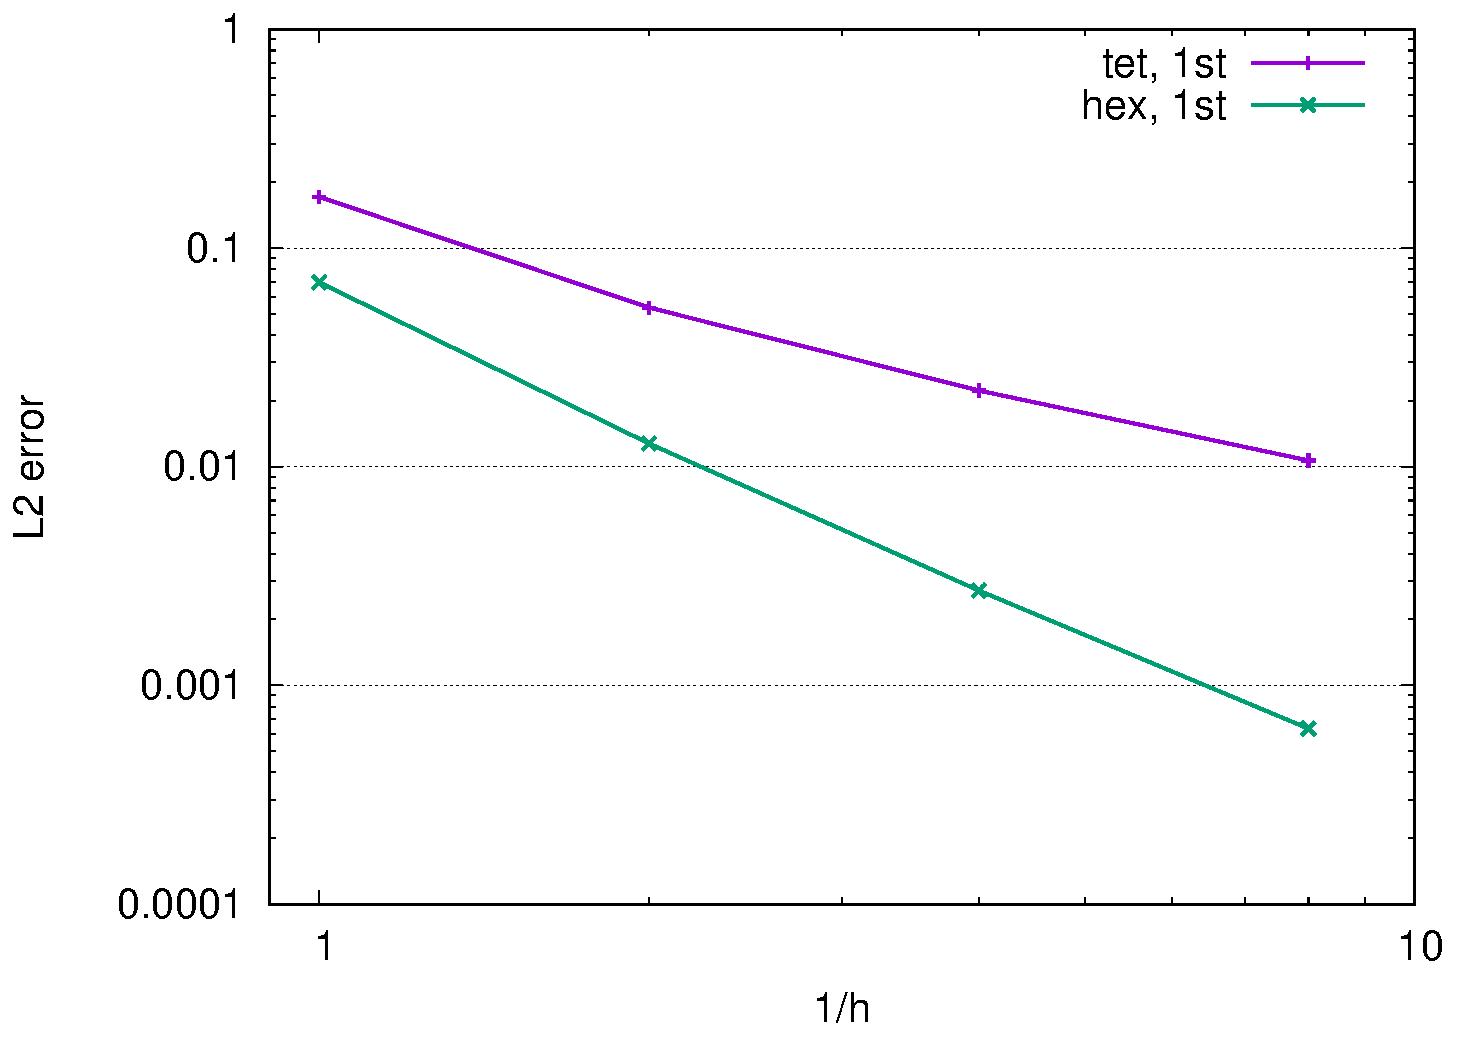
\includegraphics[width=10.0truecm]{pics/conv_convdiff_const_pe1000000.pdf}
	\caption{L2誤差: 定常・移流拡散方程式・係数一定・$\mathrm{Pe} = 1{,}000{,}000$}
	\label{fig:conv_convdiff_const_pe1000000}
\end{figure}

\subsubsection{係数非一定の移流拡散方程式}
 \label{sec:gen}
\begin{align}
	a &= 1 \\
	\bsm{v} (\bsm{x}) &= 
	\begin{Bmatrix}
		1 + x^4 \\
		1 + y^4 \\
		1 + z^4
	\end{Bmatrix} \\
	k (\bsm{x}) &= 2 + \sin x \sin \left( 0.5 y \right) \sin \left( 0.25 z \right)
\end{align}
\begin{align}
	\begin{split}
	f (\bsm{x}) &= \left( 1 + x^4 \right) \left\{ 0.25 \cos \left( 0.25 x \right) \sin \left( 0.5 y \right) \sin z \right\} \\
		& \quad + \left( 1 + y^4 \right) \left\{ 0.5  \sin \left( 0.25 x \right) \cos \left( 0.5 y \right) \sin z \right\} \\
		& \quad + \left( 1 + z^4 \right) \left\{      \sin \left( 0.25 x \right) \sin \left( 0.5 y \right) \cos z \right\} \\
		& \quad - 1.1875 \sin \left( 0.25 x \right) \sin \left( 0.5 y \right) \sin z \\
		& \quad - \left\{     \cos x \sin \left( 0.5 y \right) \sin \left( 0.25 z \right) \right\} \left\{ 0.25 \cos \left( 0.25 x \right) \sin \left( 0.5 y \right) \sin z \right\} \\
		& \quad - \left\{0.5  \sin x \cos \left( 0.5 y \right) \sin \left( 0.25 z \right) \right\} \left\{ 0.5  \sin \left( 0.25 x \right) \cos \left( 0.5 y \right) \sin z \right\} \\
		& \quad - \left\{0.25 \sin x \sin \left( 0.5 y \right) \cos \left( 0.25 z \right) \right\} \left\{      \sin \left( 0.25 x \right) \sin \left( 0.5 y \right) \cos z \right\} 
	\end{split}
\end{align}
\begin{figure}[h!!]
	\centering
	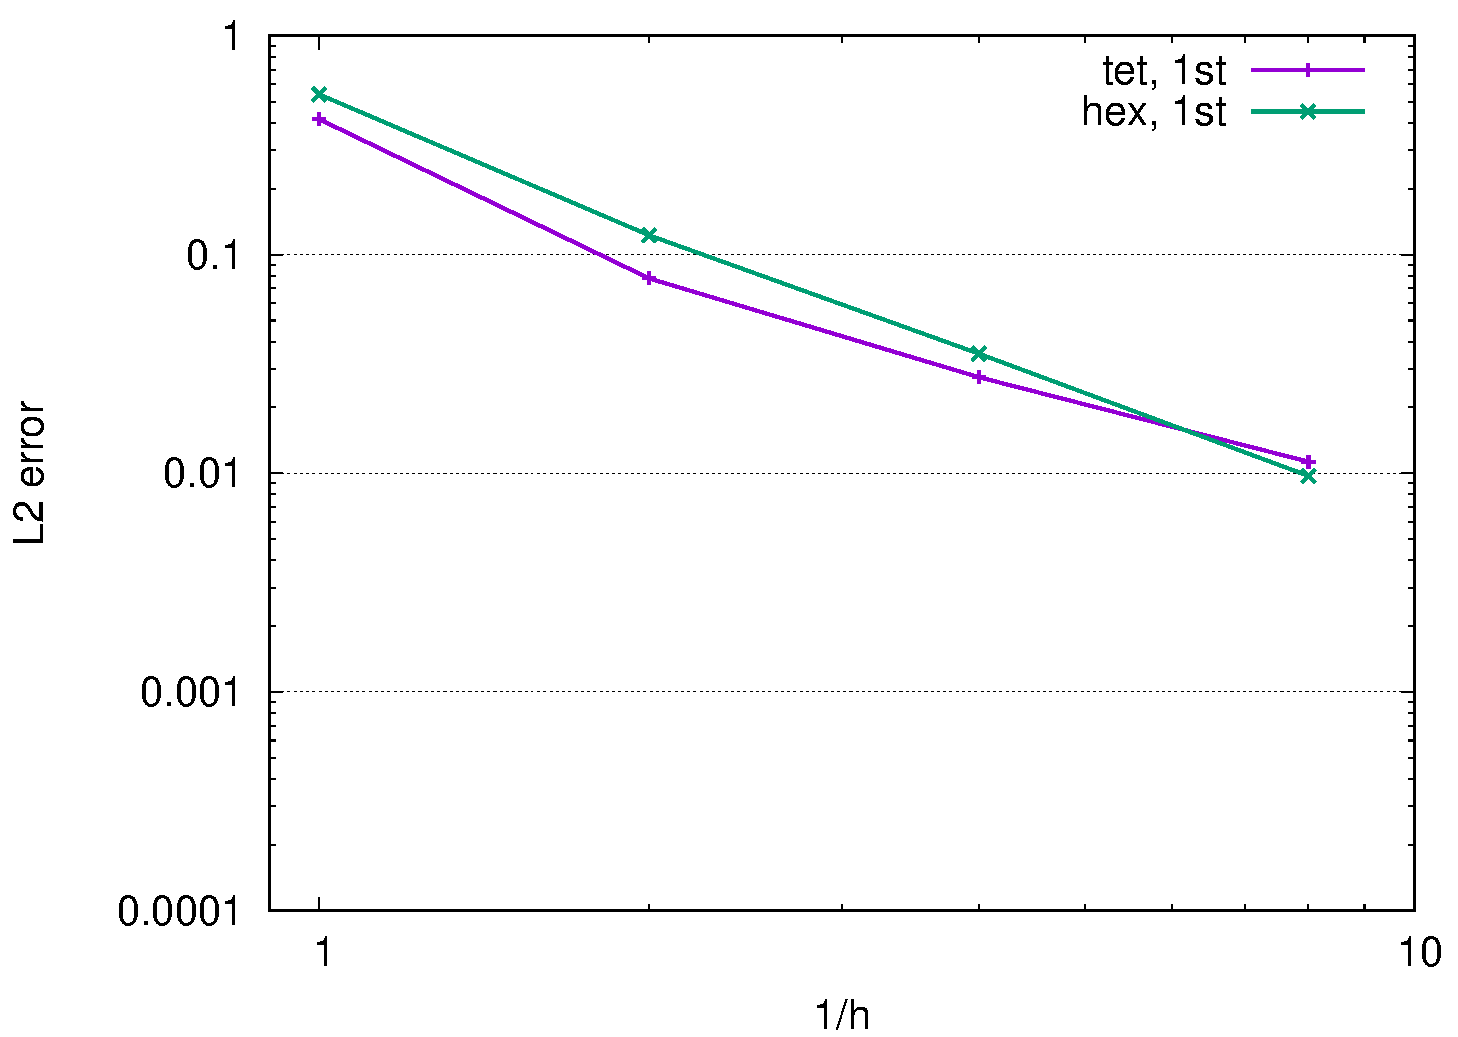
\includegraphics[width=10.0truecm]{pics/conv_convdiff_nonconst.pdf}
	\caption{L2誤差: 定常・移流拡散方程式・係数非一定}
	\label{fig:conv_convdiff_nonconst}
\end{figure}

\subsection{非定常解析}
定常解析において、有限要素法プログラムの基幹部分の検証は完了したと考えられる。
非定常解析は定常解析に対して、時間微分関連項が追加すれば実装できるため、
定常解析において最も汎用的な\ref{sec:gen}項のケースと同様の設定での検証を行う。
なお、創成解に時間依存性を導入する以外に、計算時間 (行列の反復回数低減) の観点から、移流速度の分布を変更している。

\begin{align}
	u (\bsm{x}, t) &= \sin \left( 0.25 x \right) \sin \left( 0.5 y \right) \sin z \left( 0.5 t + \sin t \right)
\end{align}
\begin{align}
	a &= 1 \\
	\bsm{v} (\bsm{x}) &= 
	\begin{Bmatrix}
		1 + x^2 \\
		1 + y^2 \\
		1 + z^2
	\end{Bmatrix} \\
	k (\bsm{x}) &= 2 + \sin x \sin \left( 0.5 y \right) \sin \left( 0.25 z \right)
\end{align}
\begin{align}
	\begin{split}
		f (\bsm{x}, t) &= \sin \left( 0.25 x \right) \sin \left( 0.5 y \right) \sin z \left( 0.5 + \cos t \right) \\
		& \quad + \left( 1 + x^4 \right) \left\{ 0.25 \cos \left( 0.25 x \right) \sin \left( 0.5 y \right) \sin z \left( 0.5 t + \sin t \right) \right\} \\
		& \quad + \left( 1 + y^4 \right) \left\{ 0.5  \sin \left( 0.25 x \right) \cos \left( 0.5 y \right) \sin z \left( 0.5 t + \sin t \right) \right\} \\
		& \quad + \left( 1 + z^4 \right) \left\{      \sin \left( 0.25 x \right) \sin \left( 0.5 y \right) \cos z \left( 0.5 t + \sin t \right) \right\} \\
		& \quad - 1.1875 \sin \left( 0.25 x \right) \sin \left( 0.5 y \right) \sin z \left( 0.5 t + \sin t \right) \\
		& \quad - \left\{     \cos x \sin \left( 0.5 y \right) \sin \left( 0.25 z \right) \right\} \left\{ 0.25 \cos \left( 0.25 x \right) \sin \left( 0.5 y \right) \sin z \left( 0.5 t + \sin t \right) \right\} \\
		& \quad - \left\{0.5  \sin x \cos \left( 0.5 y \right) \sin \left( 0.25 z \right) \right\} \left\{ 0.5  \sin \left( 0.25 x \right) \cos \left( 0.5 y \right) \sin z \left( 0.5 t + \sin t \right) \right\} \\
		& \quad - \left\{0.25 \sin x \sin \left( 0.5 y \right) \cos \left( 0.25 z \right) \right\} \left\{      \sin \left( 0.25 x \right) \sin \left( 0.5 y \right) \cos z \left( 0.5 t + \sin t \right) \right\} 
	\end{split}
\end{align}

\begin{figure}[h!!]
	\subfigure[tetrahedron element]{%
		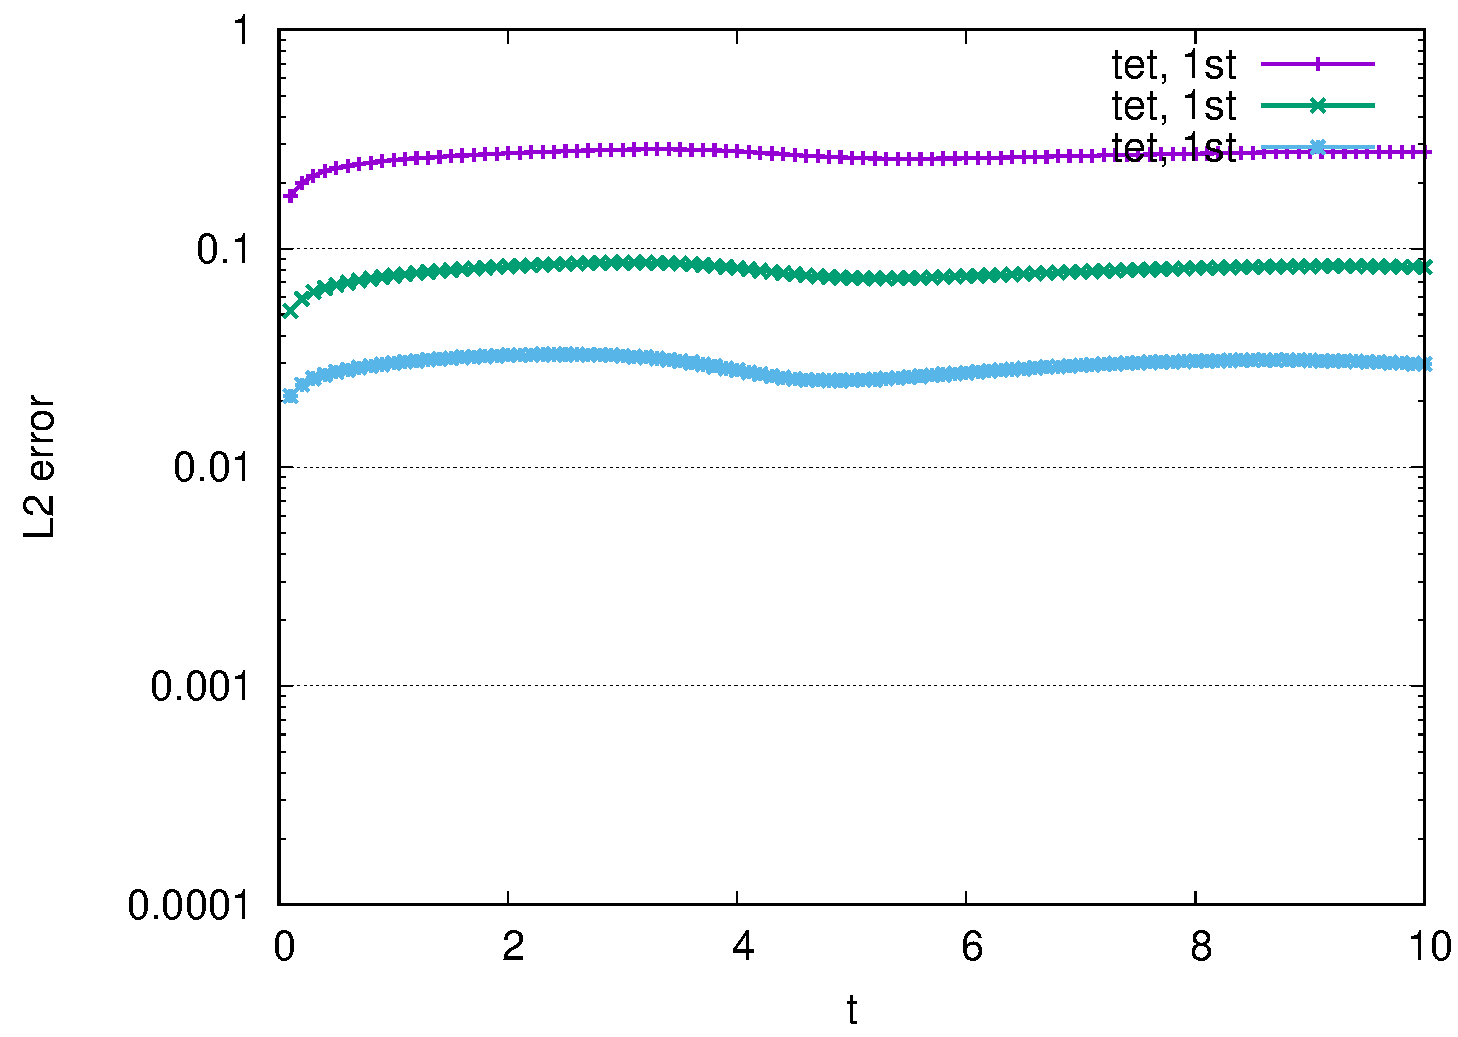
\includegraphics[clip, width=0.5\columnwidth]{./pics/l2th_convdiff_nonsteady_dt01_tet.pdf}}%
	\subfigure[hexahedron element]{%
		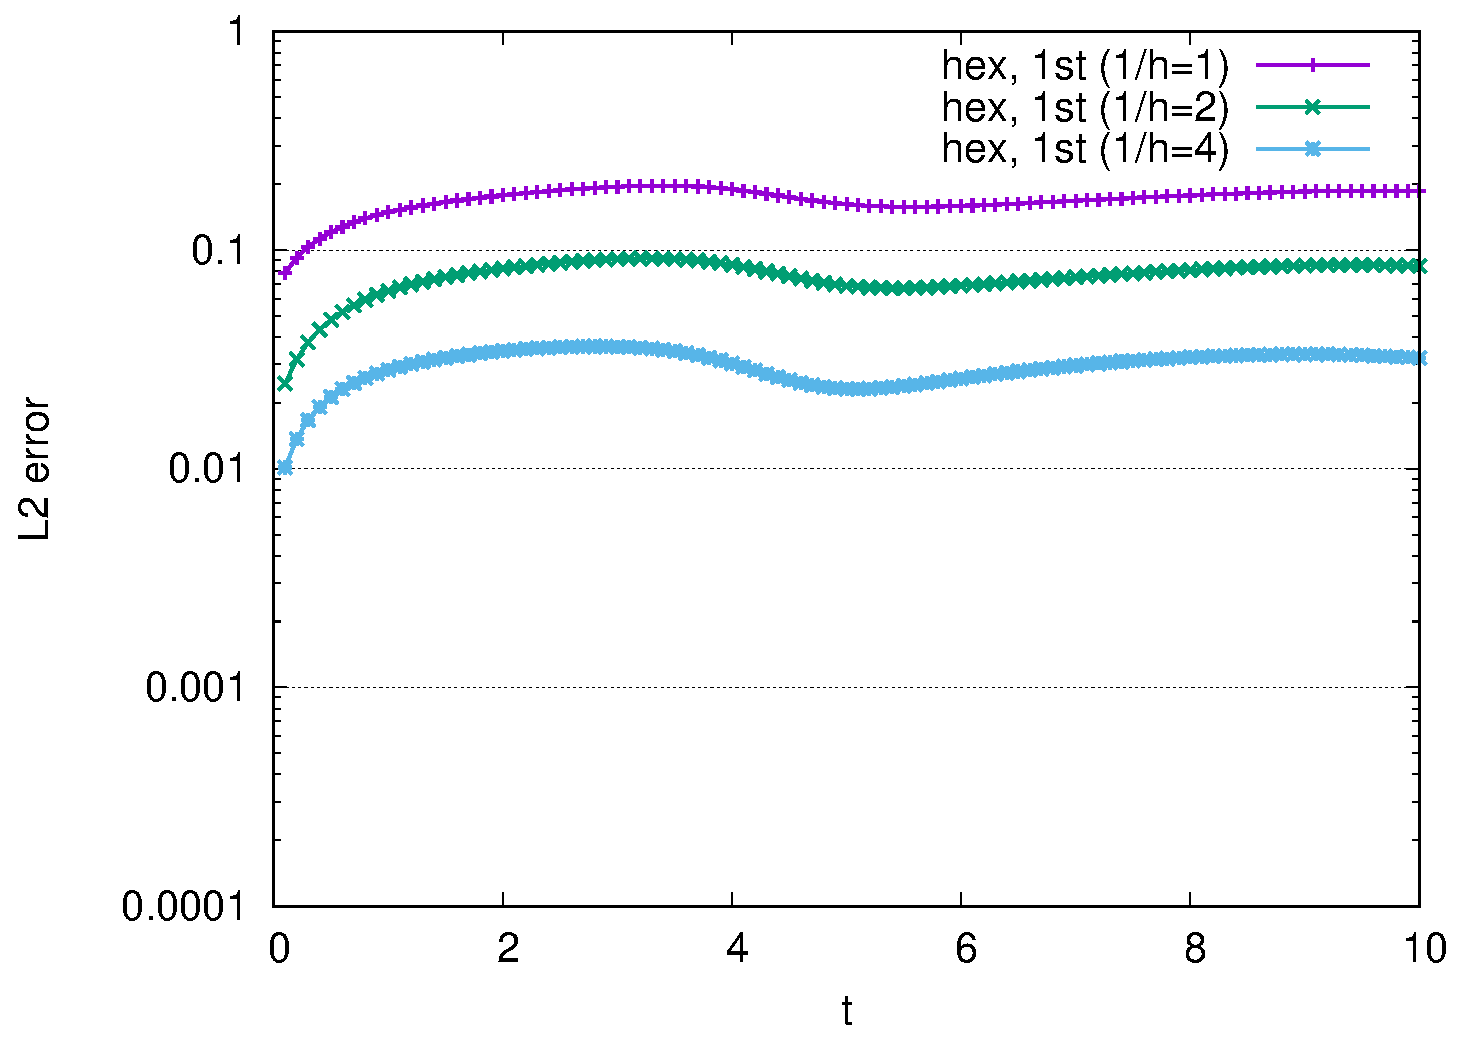
\includegraphics[clip, width=0.5\columnwidth]{./pics/l2th_convdiff_nonsteady_dt01_hex.pdf}}%
	\caption{L2誤差の時間履歴: 非定常・移流拡散方程式・係数非一定・$\Delta t = 0.1$}
	\label{fig:l2th_convdiff_nonsteady_dt01}
\end{figure}
\begin{figure}[h!!]
	\subfigure[tetrahedron element]{%
		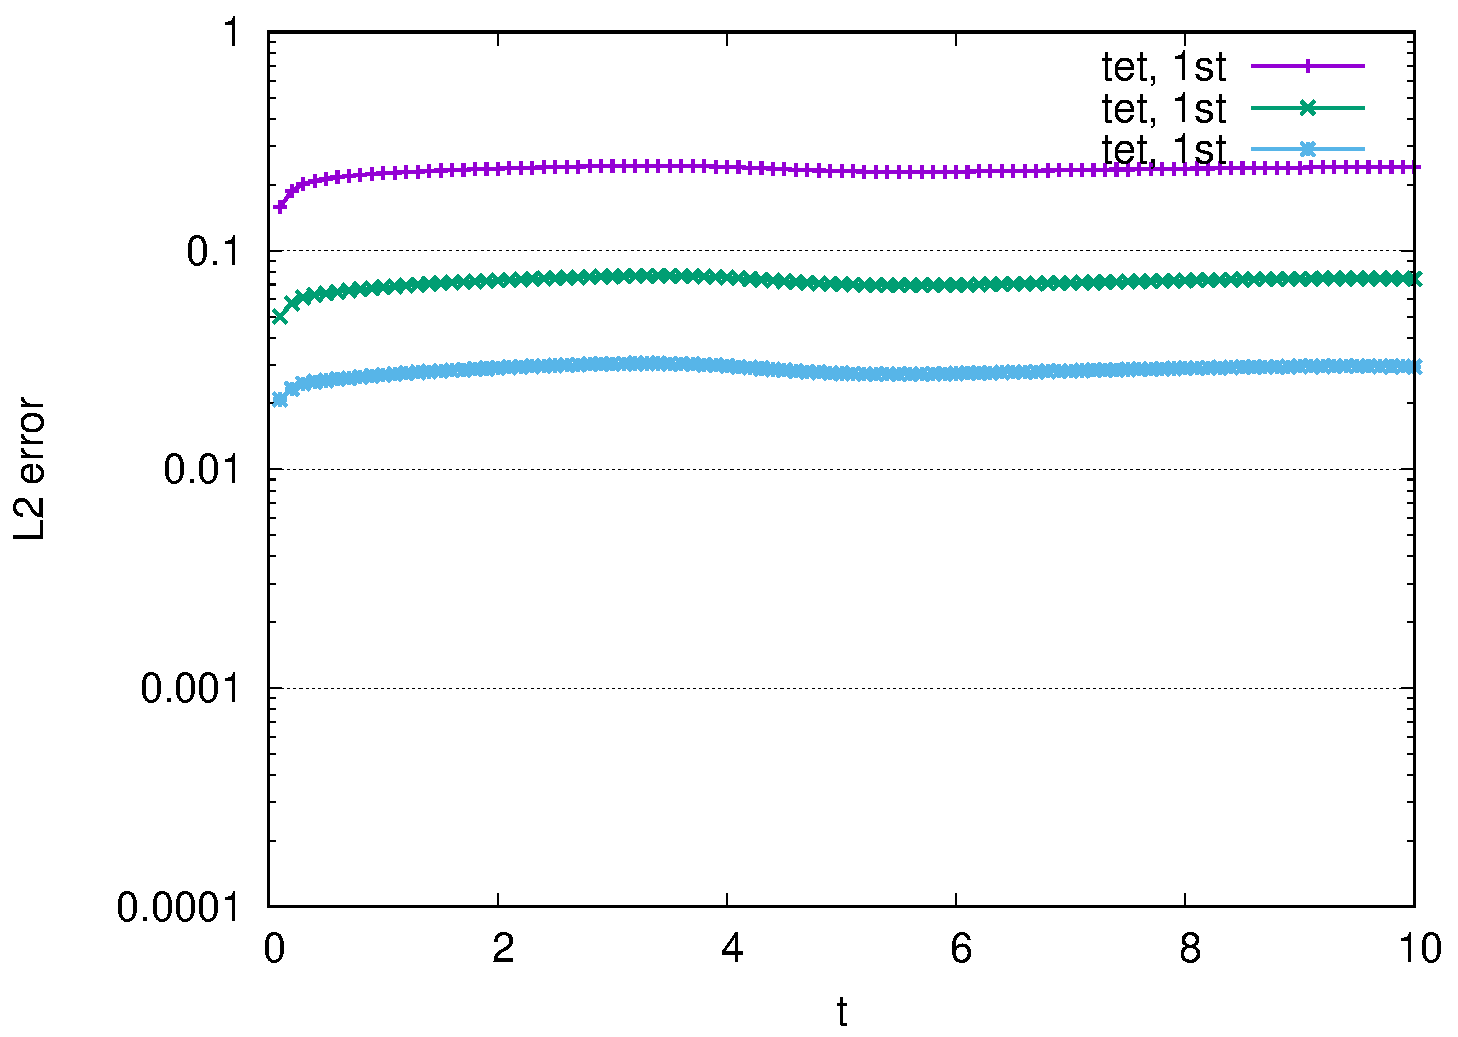
\includegraphics[clip, width=0.5\columnwidth]{./pics/l2th_convdiff_nonsteady_dt001_tet.pdf}}%
	\subfigure[hexahedron element]{%
		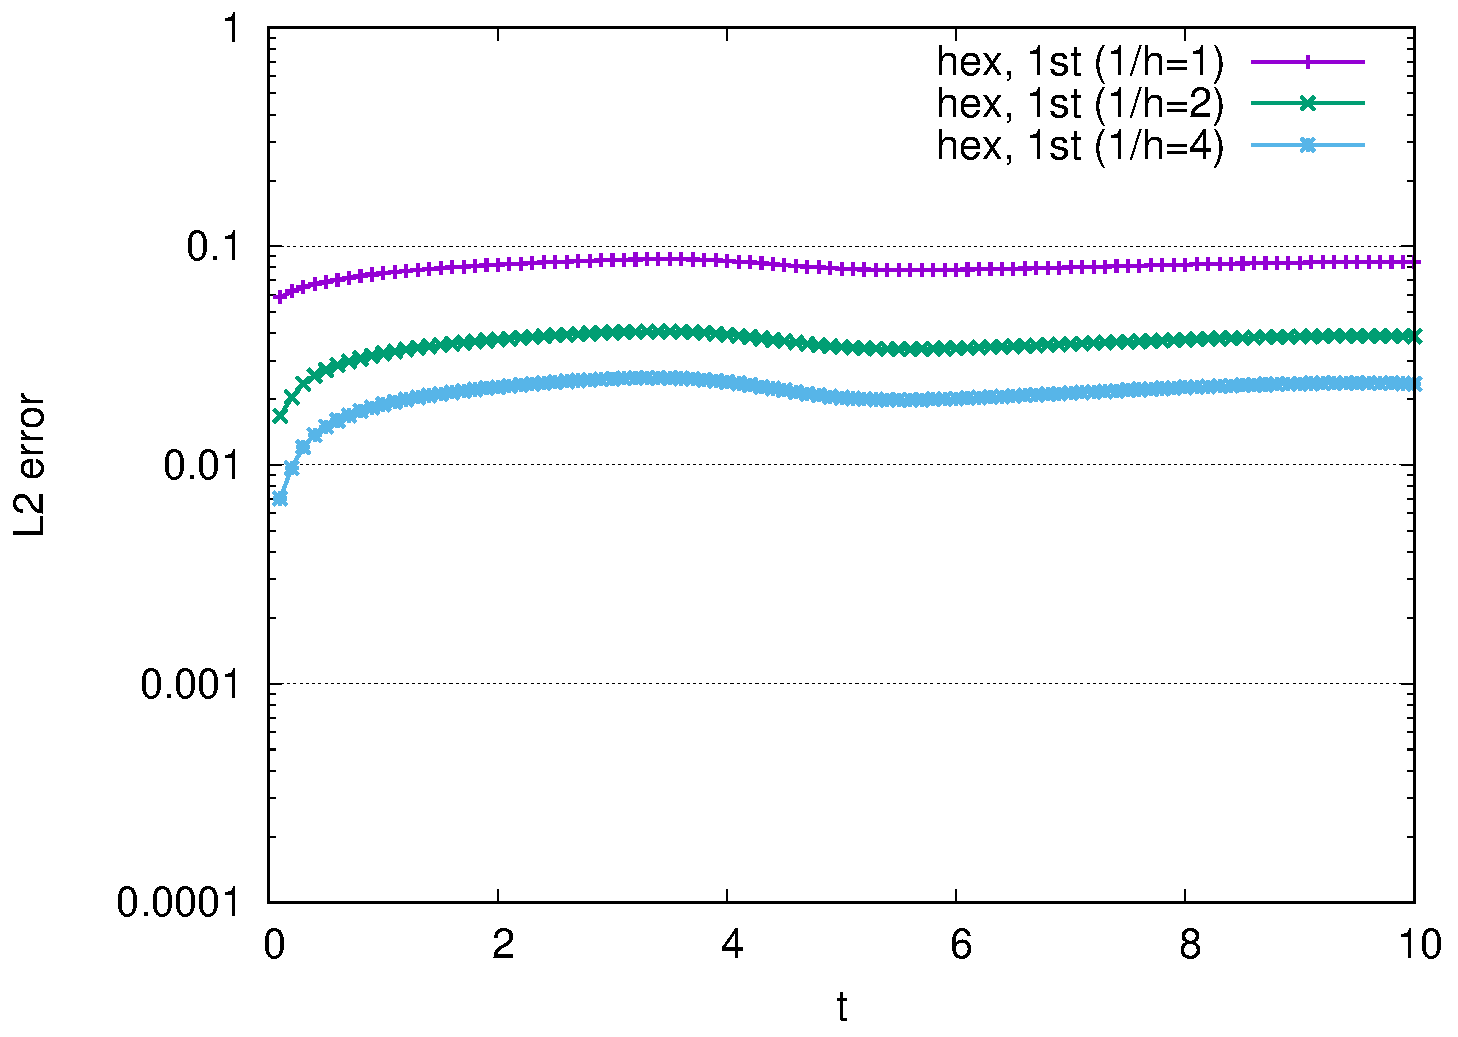
\includegraphics[clip, width=0.5\columnwidth]{./pics/l2th_convdiff_nonsteady_dt001_hex.pdf}}%
	\caption{L2誤差の時間履歴: 非定常・移流拡散方程式・係数非一定・$\Delta t = 0.01$}
	\label{fig:l2th_convdiff_nonsteady_dt01}
\end{figure}

\begin{thebibliography}{99}
	\bibitem{hughes1989new} Hughes, T.J.R., Franca, L.P., Hulbert, G.M: A new finite element formulation for CFD: VIII. The Galerkin-least-squares method for advective-diffusive equations. Computational Methods in Applied Mechanics and Engineering, 73, 173--189, 1989.
\end{thebibliography}
\end{document}

